\documentclass[12pt, a4paper]{article}

\usepackage{ctex}
\usepackage{float, booktabs, parskip, enumerate, pythonhighlight}
\usepackage{amsmath, amsthm, amssymb, mathrsfs, bm}
\usepackage{graphicx, subfigure, svg}
\usepackage{hyperref, endnotes}
\usepackage[round]{natbib}
\usepackage{multirow}

\usepackage{fontspec}
\setmainfont{Times New Roman}
\usepackage{xeCJK}
\setCJKmainfont{SimSun}[AutoFakeBold,AutoFakeSlant]
\usepackage[font={footnotesize}]{caption}
\usepackage[justification=centering]{caption}

\usepackage{geometry}
\geometry{top=3.7cm, bottom=2cm, left=2cm, right=2cm}

\usepackage{titlesec}


\setlength{\parindent}{4em}
\setlength{\parskip}{1em}
\allowdisplaybreaks[4]

\newcommand{\ivec}{\bm}

\newcommand{\NN}{\mathcal{N}}
\newcommand{\al}{\overline{\alpha}}


\title{{{\textbf{FINN：基于物理信息神经网络的城市内涝水深建模\\}}}}
\author{张景皓，钱昱诚，刘怀川，刘滨瑞}

\begin{document}

\maketitle

\begin{abstract}
洪水引发的城市内涝作为一种常见的自然灾害，对城市居民的生命和财产安全构成了持续的威胁。本文提出了一种基于U-Net、GAN，且结合水力学物理信息的神经网络模型FINN（Flood-Informed Neural Networks），可应用于城市内涝水深预测问题。实验表明，FINN在典型城市内涝场景中具备较强的水深分布建模能力，体现出了较高的预测精度与泛化能力，其推理结果与物理实际相符合。与传统数值模拟模型相比，FINN在保持较高预测质量的同时，有效地降低了计算成本，可作为代理模型部署于洪水防控工作中。我们相信，FINN在与洪水相关的水文预测问题中具有广阔的应用前景，可为未来城市内涝防治提供新的技术工具。

Urban flooding caused by heavy rainfall poses a persistent threat to the safety of residents and their property. This paper proposes a neural network model, named FINN (Flood-Informed Neural Networks), which integrates hydraulic physical information with U-Net and GAN architectures, to address the issue of urban flood depth prediction. Experimental results demonstrate that FINN exhibits strong modeling capabilities in predicting flood depth distribution in typical urban flooding scenarios, achieving high prediction accuracy and generalization ability with results that align well with physical realities. Compared to traditional numerical simulation models, FINN maintains high prediction quality while significantly reducing computational costs, making it a viable proxy model for flood prevention and control. We believe that FINN holds great potential for application in hydrological forecasting related to floods, offering new technological tools for urban flood prevention in the future.
\end{abstract}

\section{引言}

洪水是全球范围内最危险且最常见的自然灾害之一，每年都会造成重大的人员伤亡和经济损失。在城市地区，考虑到人口密集和基础设施复杂等因素，洪水带来的内涝问题显得尤为严峻。而随着气候变化进程的不断加速，更频繁、更强烈的极端降水事件将使得内涝风险进一步升级。因此，我们迫切需要更精确、更高效的预测工具来支撑未来的应急响应机制建设和城市规划工作。

\cite{bentivoglio2022deep}的调研显示，目前在城市内涝建模中主要使用三种主要洪水地图：淹没区分析地图（inundation maps）、易发性分析地图（susceptibility maps）和要素时空分析地图（hazard maps）。其中，洪水要素时空分析地图能够全面展示特定洪水事件的关键变量（如洪水深度和水域范围）的空间分布，在现代洪水灾害预防中起着最为重要的作用。为了预先得到特定洪水过程下的洪水要素时空分析地图，传统水力学研究主要使用基于流体力学的数值模拟方法。这些方法尽管准确，但在处理复杂城市地形和多变量数据时，往往计算开销巨大，实时性较差，难以部署到实际应用中。

近年来，深度学习技术在多个领域取得了突破性进展，特别是在高维数据建模和非线性模式识别方面，展现了极大的潜力。同时我们注意到，基于深度学习的建模方法相较于传统数值方法在计算速度上有着决定性的优势。因此，我们认为将深度学习方法引入水力学研究当中，特别是对于城市内涝水深预测这一重要课题，是一种创新且高效的解决方案。

我们的研究目标是将深度学习方法与传统水力学理论相结合，构建一个内嵌洪水物理过程的神经网络模型\textbf{FINN（Flood-Informed Neural Networks）}。基于静态地形参数、洪水事件中的降雨数据和入流条件，FINN将能够高效、准确地预测洪水过程中的水深分布情况，绘制出洪水要素时空分析地图。作为传统数值模型的代理，FINN对于城市内涝水深这一具体变量的端到端模拟将为城市防洪设计、风险区划定、基础设施改造以及应急决策提供关键数据支持。不言而喻，FINN不仅具有重要的科学与工程意义，还将在实际应用中带来突出的社会价值。

\section{相关工作}

\subsection{数值模型}

目前，洪水要素时空分析地图通常通过数值模型生成，这些模型通过离散化控制方程和计算域来模拟洪水事件。水动力模型是当前评估城市雨洪风险的最先进工具，并且已在多种商业软件中实现，其中以MIKE模型，HEC-RAS等为代表（\citealp{dhi2016mike}）。这些模型动态地模拟了水在地表空间和时间中的运动，并且通常与排水网络的动态模拟相结合。然而，数值模型最大的不足是其极高的计算复杂度，特别是在复杂的边界环境中。因此，数值模型在实际应用中受制诸多，应用和部署都十分不便。
    
\subsection{深度学习}

为了弥补传统数值模型的缺陷，深度学习技术已被一些学者引入了洪水要素时空分析绘图这一研究领域。大多数研究仅仅只是基于重现期的不同洪水事件概率评估，只有少量研究针对单次事件的水深分布进行了预测。

在模型架构方面，最初常使用的是多层感知机（MLP），近年来卷积神经网络（CNN）的使用正变得越来越普遍（\citealp{guo2020data}；\citealp{kabir2020deep}；\citealp{lowe2021u}）。此外，一些研究分别使用了长短期记忆网络（LSTM）和多层感知机（MLP），并结合了降阶建模框架，取得了较为不错的效果（\citealp{hu2019rapid}；\citealp{jacquier2020non}）。

我们将深度学习在城市内涝水深建模领域的优势总结为以下四点：

\begin{enumerate}

    \item 实时性与效率问题

    \par 传统数值模型通常需要高精度的地形数据、复杂的参数设置，以及大量计算资源才能得出精确结果。这对于需要快速响应的城市洪水管理场景（如极端降雨实时预警）并不适用。而深度学习通过对海量历史数据的训练，可以构建高效的预测模型，以极低的时间成本生成水深分布预测结果，从而实现快速响应。

    \item 复杂地形和多变量数据的整合

    \par 城市地形通常具有高度非线性和复杂性，涉及建筑、道路、地下排水等多层次因素。传统模型在模拟这种复杂场景时，可能会受到不确定性数据或细节不足的限制。而深度学习技术能够通过卷积神经网络（CNN）等结构直接提取地形特征，同时结合降雨强度、排水流量等多源异构数据，全面预测洪水水深。

    \item 数据稀缺性与不确定性

    \par 在许多城市，完整的洪水观测数据较为稀缺或存在较大噪声。深度学习模型可以通过迁移学习、数据增强等技术充分利用有限的样本进行高效建模，并通过不确定性量化评估预测的可靠性。

    \item 灵活性与推广能力

    \par 深度学习模型具有较强的可扩展性，一旦训练完成，可以在相似条件下应用于不同的城市区域，而不需要重新建立复杂的物理模型。
    
\end{enumerate}

值得一提的工作是\cite{lowe2021u}提出的U-FLOOD模型。U-FLOOD采用了经典的U-Net模型，以地形数据作为输入，使用MLP对水文信息进行编码，将两者在中间层隐空间内合并。U-FLOOD取得了可接受的预测结果，一定程度上证明了U-Net适用于城市内涝水深建模问题。因此，FINN也将使用U-Net作为基础架构。但是，U-FLOOD的预测仍有许多不足，其中最突出的问题是其输出结果并不符合物理实际。例如，U-FLOOD预测的总流量值往往明显大于降雨带来的总水量；在U-FLOOD给出的洪水要素时空分析地图中，显著值点过于离散而呈点状分布，这与真实世界中连续变化的洪涝水深相比相去甚远。我们认为，这些问题是由于U-FLOOD没有考虑水力物理约束所致，其预测结果的置信度也因此亟待考量。

\section{问题定义}

在已有相关工作的基础上，FINN将聚焦于解决以下若干关键问题。

\subsection{如何构建内嵌洪水物理过程的神经网络模型}

构建内嵌洪水物理过程的神经网络模型需要将物理知识与深度学习方法相结合，以增强模型对实际洪水过程的模拟能力。FINN采取的具体实现方法是物理约束的正则化应用：在模型的损失函数中引入物理约束。通过在训练过程中施加这些物理约束，我们可以确保FINN的输出将更加符合实际的物理现象。

\subsection{如何进一步提高城市内涝水深建模的精度}

为了提高城市内涝水深建模的精度，关键在于进一步优化模型结构，增大数据量和参数量，从而提高模型的泛化能力。
在U-Net的基础架构之上，FINN还采用了生成对抗网络技术（GAN）。另外，相较于同类模型，FINN进一步提高了参数量，并进行了充分的超参数搜索调优。通过上述改进，我们期望FINN能够提供更高精度的城市内涝水深预中结果。

\section{模型构建}

\subsection{数据}

我们的研究区域位于丹麦城市Odense。我们从丹麦地理数据门户网站获得了城市地形数据，其中研究区域为$3740\times 4273$的像素点，其中每个像素点的分辨率为5m。每个像素点有若干地形数据，我们选取了其中6个作为模型输入。
\begin{table}[htbp]
    \centering
    \begin{tabular}{|c|l|}
    \hline
    \textbf{变量名} & \multicolumn{1}{c|}{\textbf{变量含义}} \\
    \hline
    $curv$ & 表征地形的凹凸，归一到$[0,1]$。 \\
    \hline
    $imp$ & 每个像素点的不透水性，范围在$[0,1]$。 \\
    \hline
    $slope\_flacc\_w$ & 像素点的汇水面积，上限为250ha。 \\
    \hline
    $sinkdepth$ & 淹没水深，为像素点出流处高程与像素点高程之差，至少为0。 \\
    \hline
    $cos$ & 流向角度的$cos$值。 \\
    \hline
    $sin$ & 流向角度的$sin$值。 \\
    \hline
    \end{tabular}
    \caption{地形数据变量解释}
    \label{t1}
\end{table}

对于降水数据，我们根据当地雨量计观测结果，选取了43个高强度降雨事件和10个中小型降雨强度事件，原始的降雨数据为逐小时降雨量的时间序列。我们进行了特征提取，选取了9个特征作为模型输入。
\begin{table}[H]
    \centering
    \begin{tabular}{|c|l|}
    \hline
    \textbf{特征名} & \multicolumn{1}{c|}{\textbf{特征含义}} \\
    \hline
    $dur$ & 降雨事件历时。 \\
    \hline
    $P_{tot}$ & 降雨事件的总降雨量。 \\
    \hline
    $r_p$ & 降雨峰值相对于事件总持续时间的时间索引。 \\
    \hline
    $r_{cg}$ & 中位累积降水量相对于事件总持续时间的时间索引。 \\
    \hline
    $m_1$ & 降雨峰值前后的累积降水量比率。 \\
    \hline
    $m_2$ & 最大降雨强度（10分钟间隔）与总降水深度的比率。 \\
    \hline
    $m_3$ & 事件开始前三分之一的降水深度与总降水深度的比率。 \\
    \hline
    $m_5$ & 事件开始前半部分的降水深度与总降水深度的比率。 \\
    \hline
    $n_i$ & 最大降雨强度（10分钟间隔）与平均降雨强度的比率。 \\
    \hline
    \end{tabular}
    \caption{降雨特征解释}
    \label{t2}
\end{table}

我们使用MIKE21模型进行二维水动力洪水模拟，将模拟结果作为模型的标准输出。

\subsection{模型架构}

为了更加准确地预测不同降雨情况内的城市内涝洪水水深，我们搭建了多种模型并将其进行测试与对比。首先，我们依据过往研究中对于该问题的深度学习方法，在本案例中进行结果复现。由于这类问题需要预测空间范围内的水深指标，深度学习方法下的主流习尝试是基于UNet或其变种进行的，在多个案例上都取得了相对较好的结果\endnote{Guo Z, Leitao J P, Simões N E, et al. Data‐driven flood emulation: Speeding up urban flood predictions by deep convolutional neural networks[J]. Journal of Flood Risk Management, 2021, 14(1): e12684.}$^,$\endnote{Löwe R, Böhm J, Jensen D G, et al. U-FLOOD–Topographic deep learning for predicting urban pluvial flood water depth[J]. Journal of Hydrology, 2021, 603: 126898.}。接着，我们在UNet的基础上加入物理与统计机制的约束,在损失函数上加入水量与空间连续性的惩罚项，组成Physical-Informed UNet(PI-UNet)，在进一步提升模型在预测内涝表现的同时也增加了其可解释性。最后，我们创新性地将UNet与生成对抗网络(Generative Adverse Network, GAN)结合为UNet-GAN，利用GAN在学习和生成具空间特征分布数据的优越性，进一步改进了前两种UNet在预测的洪水分布上与结果差异较大的短板,在实现替代传统水动力学预测模型上更进一步。

\subsubsection{UNet}

UNet是一种用于图像分割的卷积神经网络（CNN），首次由Olaf Ronneberger等人于2015年提出\citep{ronneberger2015u}。该网络最初设计用于生物医学图像的分割任务，并在在细胞图像分割与识别中表现出色。UNet相较于其它网络的的特点是其对称的U形结构。空间数据通过编码器压缩为维度更低的通道数据，并通过解码器从通道复原回原始图像。编码器与解码器之间通过跳跃连接保留图像信息，使解码器输出的结果保留原图像的部分特征。该结构
令UNet能有效学习空间数据，并且在重建过程中保持细节，特别是边缘、梯度和其他关键结构。

在城市洪涝预测的案例中，内涝水深这一变量很大程度上依赖对于空间信息的结构，如城市地形的梯度和坑洼程度等，这与UNet网络架构上学习的问题很相似。另一方面，内涝水深也与降雨时间本身高度相关。单次降雨事件中的降雨过程曲线不同，其雨强、降水分布与持续时间均不同，会导致截然不同的积水结果。因此，模型输入也要考虑降雨的各种特征(见3.1)。我们部分参考了文献中对于降水特征的输入，对于一条提取特征后的9维降雨数组，我们通过一个线性层将其映射为高维数组(4096维度)，将其重塑为与隐空间宽高相同的结构(16$\times$16$\times$16)，并将其连接到被UNet编码后的图像组内,与之一同进行解码。整体模型结构如图\ref{unet}所示。

\begin{figure}[htbp]
    \centering
    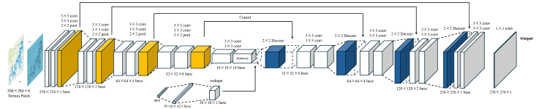
\includegraphics[width=1.0\columnwidth]{./assets/unet_struc.png}
    \caption{UNet架构}
    \label{unet}
\end{figure}

\subsubsection{具物理信息建模的PI-UNet}

UNet对图像的整体信息控制较好，可以生成与降雨-地形信息相匹配的总体误差较小的实验结果。然而，UNet在结果可解释上并不优秀，其在测试集上生成的内涝图的水深分布仍无法完全匹配坑洼的基本结构，且水深输出值并非均为正。这些问题反映了UNet作为纯数据驱动模型在物理信息学习上的缺陷。因此，本研究中参考物理机制神经网络(Physics-Informed Neural Networks, PINNs)，通过修改UNet架构的损失函数,引入两种物理机制的惩罚项,增强UNet的物理信息建模能力。

基于物理信息的神经网络最早由Maziar Raissi等人于2017年提出\citep{raissi2017physics}，旨在将物理方程与深度学习模型结合，以解决深度学习对于某些复杂物理问题中无法反映物理机理的局限性。PINN将偏微分方程（PDE）等物理规律作为约束条件引入到神经网络的损失函数中，从而使神经网络不仅能从数据中学习到模型输出，还能够遵循已知的物理约束。目前，PINN在多个领域被尝试应用。在流体动力学领域，PINN能将一维的扩散方程或二维的纳维-斯托克斯流体方程以差分形式写入损失函数中，从而在模拟流体流动、气候变化、空气动力学等复杂流体问题中占有优势。目前，部分PINN兼具推理快速、结果相对精确和可解释性的优势，已经能作为数值仿真的替代模型。

在本研究中，受限于UNet中卷积层无法完成微分节点的计算和输出，因而无法准确控制流体在空间上的运动规律。本组遂在损失函数上加入水量平衡和空间连续性这两个层面的惩罚项，引导模型关注概化的物理机制，从而获得可理解的输出结果。惩罚项的添加如下伪代码：

\begin{python}
# 基础惩罚项：基于MSE的惩罚
Loss = MSEloss(预测图像, 真实图像)
# 基于水量平衡原理的惩罚项
Loss += C_material * (预测总水量 - 降雨总水量 * 0.03) ** 2 
# 基于空间连续性的惩罚项
Loss += C_dynamics * (预测值图像梯度 - 实际值图像梯度) ** 2 
\end{python}

水量平衡原理的惩罚项是基于区域水文过程上的径流量等于总降雨量减去总蒸发量和净出流量的统计学原理。为了概化总蒸发量和净出流量在水量平衡中的数额，本组分析了测试集中145个降雨情形下流域区块的总水深和总降雨的关系，得到换算的概化水量平衡关系：
\begin{equation}
    Q \approx 0.03 \times P
\end{equation}
式中：$Q$为预测水量(水深)，$P$为降水量(水深)。

将这一关系以差分的形式计算损失，并通过二次项($L2$形式)平滑化以方便反向求导，得到基于水量平衡原理惩罚项的基础形式。

空间连续性的惩罚项是考虑到积水边界与水深特征的情况。对于不同类型的区域上，积水边界和水深变化是建模内涝的重要物理特征。在没有约束时，UNet输出的结果普遍偏平滑，全空间上的水深差异较小(见4.2.2推理结果)。因此在物理机制引入时，我们将这一因素纳入损失函数中重点关注，通过计算预测值图像梯度与真实梯度之间的$L2$差异，得到基于空间连续性惩罚项的形式。

\subsubsection{具空间分布生成的UNet-GAN}

UNet虽然可以很好地处理并学习图像信息，但是其对于内涝水深分布的生成任务有天然的不足。受限于损失函数的指导只能局限于对图像上所有像素的误差统计,UNet在根本原理上无法准确捕捉水深的分布情况。因此，借鉴于生成模型对于学习分布的优越性特点，本研究创新性地利用生成对抗网络(GAN)做基础架构，改造UNet成为合适的生成器并使其在对抗中进一步强化对城市内涝水深分布的学习。

生成对抗网络最早由Ian Goodfellow等人于2014年提出\citep{goodfellow2014generative}，是一种基于对抗学习的生成模型。与前述VAE模型不同，GAN旨在更直接地解决生成模型的生成器无法生成优秀图像的问题。GAN将博弈论(Game Theory)的思想引入模型结构中，采用“生成-监督”的对抗策略进行迭代，从而期望模型达到以假乱真的效果。

GAN的结构如图2所示。其含有一个生成器$G$(Generator)，通过从样本空间内的噪声$z$生成$G(z)$的结果；同时一个判别器$D$(Discriminator)可以学习并判别出给定样本属于自然样本而非生成器生成样本的概率。因此在GAN的优化中，一方面要使生成器$G$尽可能做到以假乱真，另一方面也要使判别器$D$可以明辨真假，从而在下一轮对抗中对$G$提出更高的要求。

GAN采用的损失函数$V(D, G)$如下：
\begin{equation}
    V(D, G) = \mathbb{E}_{x\sim p_{data}(x)} [log(D(x))] + \mathbb{E}_{z\sim p_{z}(z)} [log(1-D(G(z)))]
\end{equation}

其中，第一项为以服从原始采样分布下判别器$D(x)$的表现，由于$x$均为$data$内自然样例，此时对每个样点$x$，$D(x)$应显示尽可能高的概率；而第二项为以服从某个噪声分布$p_{z}(z)$下生成器与判别器的表现，对于判别器$D$，应尽可能分辨生成器生成的样本，因此$D(G(z))$要尽量小，反之对于判别器，要做到以假乱真因此需要$D(G(z))$尽量大。$x$与$z$分别代表着正确例与错误例，思路上类比交叉熵损失函数采用$log(\hat{y})$与$log(1-\hat{y})$求和。

在本研究中，我们以在前两个模型中搭建好的成熟的UNet作为生成器$G$, 以一个五层卷积层的简单神经网络作为判别器$D$，卷积层之间通过$LeakyRelu$函数相连接。在二、三、四层之间进行批量归一化(BatchNormalize)，使参数在神经网络层之间稳定传递。这些方法都用以保障求导时梯度不会爆炸和消失。UNet-GAN的架构如图\ref{ugan-fig}所示。

\begin{figure}
    \centering
    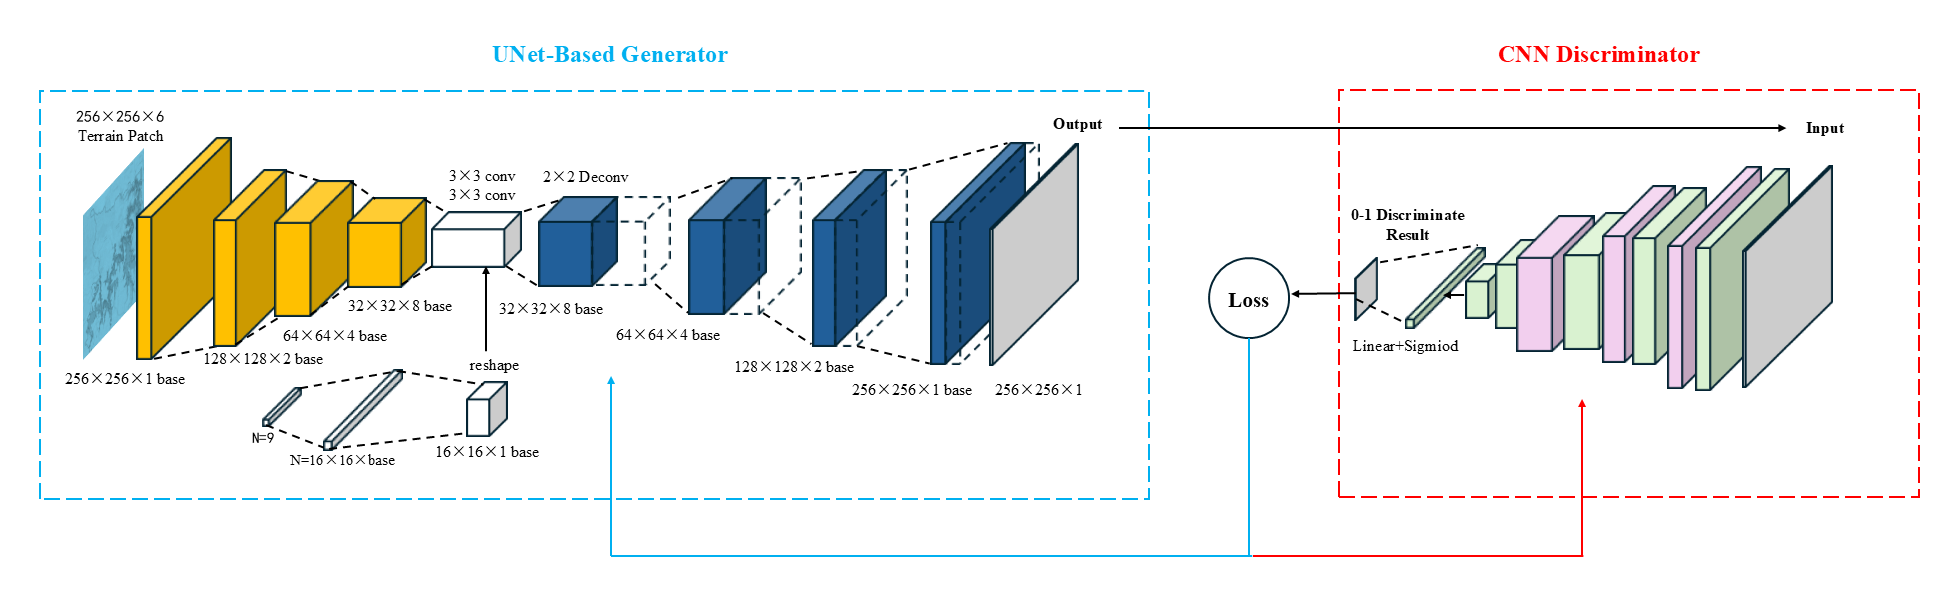
\includegraphics[width=1.0\columnwidth]{./assets/ugan2.PNG}
    \caption{UNet-GAN生成对抗模型架构图}
    \label{ugan-fig}
\end{figure}

\section{实验}

\subsection{实验设置}

\subsubsection{数据}

研究区域如图所示，我们将研究区域划分为了119个子区块，每个子区块为$256\times 256$的像素点。我们随机选择了29个子区块和5个降水事件，得到145组测试集数据。对剩余的区块和降水事件，我们进行重采样，其中区块的采样大小同样为$256\times 256$像素点，要求采样区块位于研究区域内，且不能涉及测试集的子区块，但可以与原先划定的区块不重合。我们得到了10000组“区块-降水”对，划分其中$90\%$的数据为训练集数据，其余$10\%$为验证集数据。

\begin{figure}[htbp]
    \centering
    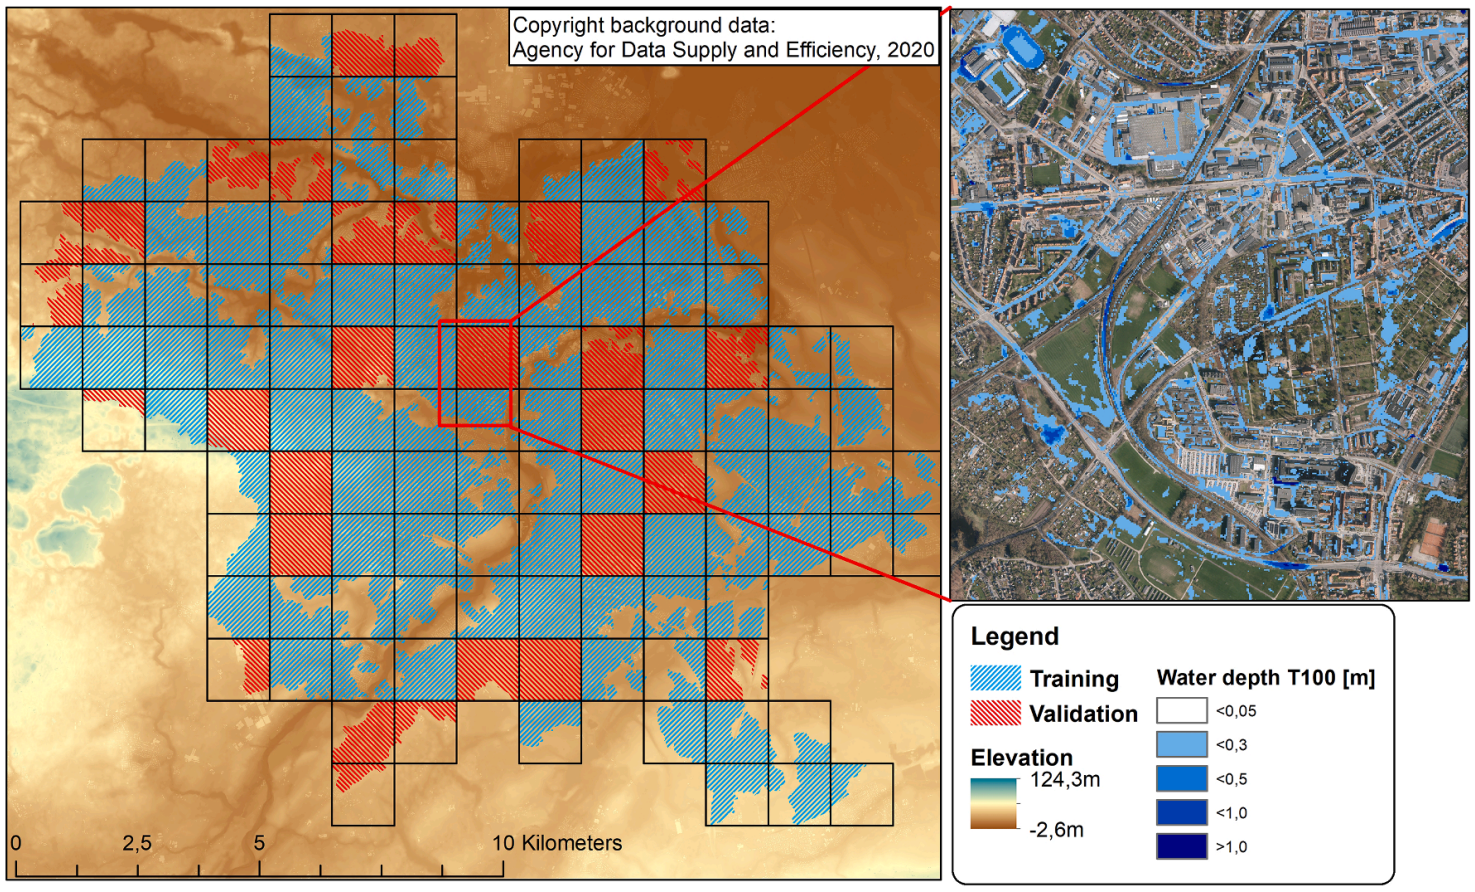
\includegraphics[width=0.8\columnwidth]{./assets/study_area.jpg}
    \caption{研究区域示意图}
    \label{area}
\end{figure}

\subsubsection{超参数}

在超参数的选择上，本研究中重点调整了模型学习层面的超参数，如学习率、学习策略等，而对模型架构层面的超参数(如层数、通道数等)进行固定。在解决内涝问题的情景下，我们所使用的三个模型均以UNet作为模型或模型基础，其架构是对\cite{lowe2021u}所使用的UNet模型的复现。在该论文中，初始通道数固定设置为64，编码器与解码器的层数固定为4层，前后两个编码或解码层在升降维的基础上以2倍通道数递增或递减,这也是常规UNet的布置方式。

对于学习率、学习策略和迭代次数，本研究通过设置不同超参数情形进行逐一实验，在原始模型上确定了本案例UNet架构的最佳学习率与基本收敛时的迭代次数,并在UNet和PI-UNet两个模型的实验中保持了这一学习率。对于UNet-GAN而言，由于生成对抗时损失函数难以收敛，需要重新实验获得可收敛的学习率。学习策略上，本研究采用带预热的余弦退火法进行优化。在训练初期，学习率会经过从0开始增加的线性预热过程，以避免前期训练不稳定的情况。预热阶段结束后，学习率进入余弦退火阶段，按照余弦函数变动以帮助模型在后期更好地收敛。预热期的长度设置为总迭代次数的$1/20$。

我们在UNet主架构中完成了学习率从$[5\times10^{-6}, 3\times10^{-4}]$之间的测试，不同学习率下模型在训练集与验证集上的$R^2$指标如图\ref{train_r2_unet_lr}和图\ref{val_r2_unet_lr}所示。由结果可知，模型在$[5\times10^{-5}, 1\times10^{-4}]$下指标表现最好，训练集和验证集的$R^2$可达到$0.55$左右。因此选择在这一指标范围内作为UNet最优学习率曲线，在UNet和PI-UNet上展开性能评估。此外，我们通过一次长程迭代学习确定模型在训练集上的损失函数收敛位置为500次迭代，指标稳定的位置为2500次迭代。综合选择模型的训练迭代次数为4000次。

\begin{figure}
    \centering
    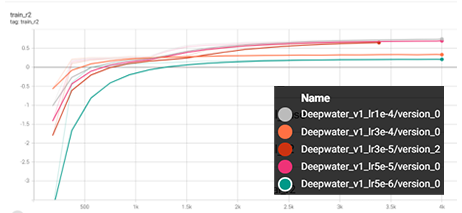
\includegraphics[width=0.8\columnwidth]{assets/train_r2.png}
    \caption{不同学习率下模型在训练集的指标图像}
    \label{train_r2_unet_lr}
\end{figure}

\begin{figure}
    \centering
    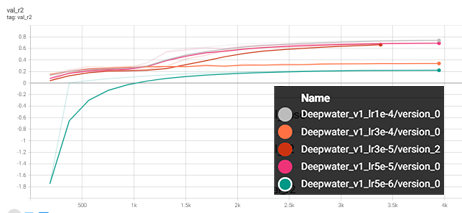
\includegraphics[width=0.8\columnwidth]{assets/val_r2_3.png}
    \caption{不同学习率下模型在验证集的指标图像}
    \label{val_r2_unet_lr}
\end{figure}

\subsubsection{指标}

我们使用$MSE$、$MAE$、$R^2$和$LPIPS$四个指标测试模型的性能，$MSE$、$MAE$和$R^2$定义为：

\begin{align}
MSE=\sum_{i=1}^{N}\sum_{j=1}^{N}(y_{i,j}-\hat{y}_{i,j})^2 \\
MAE=\sum_{i=1}^{N}\sum_{j=1}^{N}|y_{i,j}-\hat{y}_{i,j}| \\
R^2= 1-\frac{\sum_{i=1}^{N}\sum_{j=1}^{N}(y_{i,j}-\hat{y}_{i,j})^2}{\sum_{i=1}^{N}\sum_{j=1}^{N}(y_{i,j}-\overline{y}_{i,j})^2}
\end{align}

式中：$y,\hat{y}$分别为MIKE21计算结果和神经网络模型计算结果。

指标$LPIPS$的全称为$Learned\ Perceptual\ Image\ Patch\ Similarity$，该指标预训练了一个卷积神经网络，这个神经网络将输入的图像处理为若干特征向量。指标通过计算两个图像处理后特征向量的加权距离，反映这两个图像的相似度，$LPIPS$值越低表示两个图像越相似。$LPIPS$在构建网络时考虑了人类视觉系统对图像的感知，评价标准更符合人类直觉。

当然，模型在某一指标上表现得更好，并不意味着该模型一定学习到了更多的信息。传统指标$MSE$、$MAE$和$R^2$更加关注图像的平均差值，因此网络可能通过对图像整体值的加减得到更优的指标，但这显然是不合理的，事实上区块中的多数位置是没有洪水的，水深就应该是0，而不是一个偏移后的值。此外，传统指标并没有关注图像相邻像元的大小关系，可能导致结果斑块化。

\subsection{性能评估}

\subsubsection{模型训练与收敛情况}

UNet和PI-UNet的模型训练通过反向传播优化UNet架构，损失函数的收敛情况如图所示。不同学习率下UNet损失的收敛值基本一致,在$[1\times10^{-3}, 2\times10^{-3}]$之间。表明UNet本身的收敛情况较好；PI-UNet同样容易收敛，但是由于添加了两个的概化物理机制损失项，其最终的收敛值也增大到$5\times10^{-3}$左右。

对UNet-GAN而言，其训练与收敛情况更加复杂。由于受限于生成对抗网络自身的梯度不稳定情况，实际训练时UNet-GAN十分容易造成模型不收敛或生成判别器损失值消失的问题。研究中独立调整了架构中UNet生成器和CNN判别器的学习率,并设置训练策略为每优化1次生成器,同步地优化2次判别器以补足CNN在模型复杂度上的劣势。经过优化后的UNet-GAN可以实现模型在2500迭代次数范围内进行对抗学习，并使得生成器UNet产生更可信的结果，如图\ref{gan_loss_fig}所示。

\begin{figure}[htbp]
\centering
\subfigure[UNet生成器训练曲线]{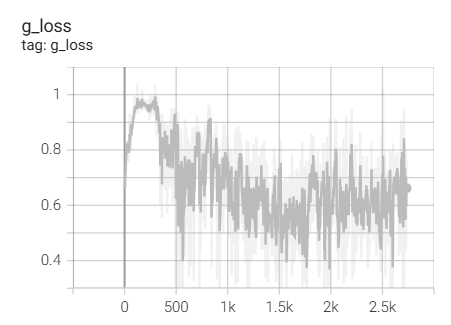
\includegraphics[width=0.40\columnwidth]{./assets/gan_g_loss.png}}
\subfigure[CNN判别器训练曲线]{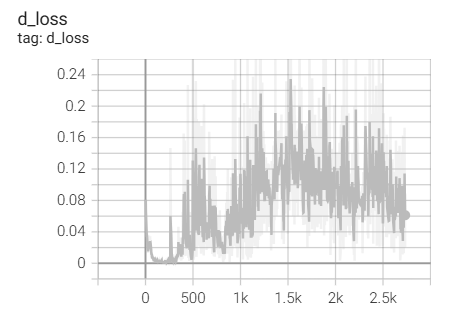
\includegraphics[width=0.40\columnwidth]{./assets/gan_d_loss.png}}
\caption{UNet-GAN训练收敛曲线图}
\label{gan_loss_fig}
\end{figure}

\subsubsection{测试指标结果}

将每一种模型在最优超参数下进行测试和推理，通过指标和具体区域上的水深预测结果来反映模型在城市内涝预测上的性能。

在测试集上，测试预测值与真实值的$MSE$、$MAE$、$R^2$与$LPIPS$，测试结果如表\ref{chat_res}所示。所有模型在指标上的差距并不显著。从指标上分析，UNet在均方根误差$MSE$与平均绝对误差$MAE$上表现均最好,分别达到了0.0017以及0.008。PI-UNet在$R^2$上得到的最高分数为-0.006。对于反映空间分布的指标$LPIPS$，则是UNet-GAN的差异程度最小，为0.5724。需要指出的一点是，在内涝水深预测这一案例中，三种指标仅能部分反映模型的预测性能。内涝只集中在空间中很小一部分的易感区域，而其它未内涝的区域的真值均为0。而模型在预测时可能将整个空间的值以接近0的指标预测，虽然对内涝水深不敏感，但也能使$MSE$、$MAE$达到可被接受的范围。$R^2$由于同时考虑了预测值与真值的误差以及真值序列的差异，相较于$MSE$和$MAE$而言更难“作弊”，因此各模型在$R^2$上都没有获得优秀的分数。$LPIPS$则通过网络层概化地反映了预测值与真值的分布差异，在这一任务上也能更加灵敏地判别模型的表现。

\begin{table}[h!]
  \begin{center}
    \begin{tabular}{lllll} % <-- Alignments: 1st column left, 2nd middle and 3rd right, with vertical lines in between
    \hline
      \textbf{Model} & \textbf{$MSE$} & \textbf{$MAE$} & \textbf{$R^2$} & \textbf{$LPIPS$}\\
      \hline
      UNet & \textbf{0.0017} & \textbf{0.008} & -0.027 & 0.6230\\
      PI-UNet  & 0.0040 & 0.024 & \textbf{-0.006} & 0.6187\\
      UNet-GAN & 0.0039 & 0.009 & -0.023 & \textbf{0.5724}\\
    \end{tabular}
  \end{center}
  \caption{模型指标结果表}
  \label{chat_res}
\end{table}

从指标角度来看，UNet在$MSE$和$MAE$上表现最佳，PI-UNet在$R^2$上稍有优势，而UNet-GAN在$LPIPS$上显示出最小的空间分布差异。然而，由于内涝水深主要集中在易感区域和大部真值为零的分布，$MSE$和$MAE$无法充分反映模型性能。$R^2$更能真实反映模型预测的准确性，而$LPIPS$则在评估空间分布差异上具有较高的敏感度。对于模型的真实预测性能而言，需要结合推理结果才能更清晰地加以阐释。

\subsubsection{推理结果}

预测的结果通过规范化处理后，消隐其中的小值像素为0(以默认其不会产生内涝)。不同模型的预测结果与真实结果如图\ref{res_1}和图\ref{res_2}如示。两张图中，左上对应于水深的真实值；右上对应于UNet的预测;左下对应于PI-UNet的预测;右下对应于UNet-GAN的预测。

\begin{figure}
    \centering
    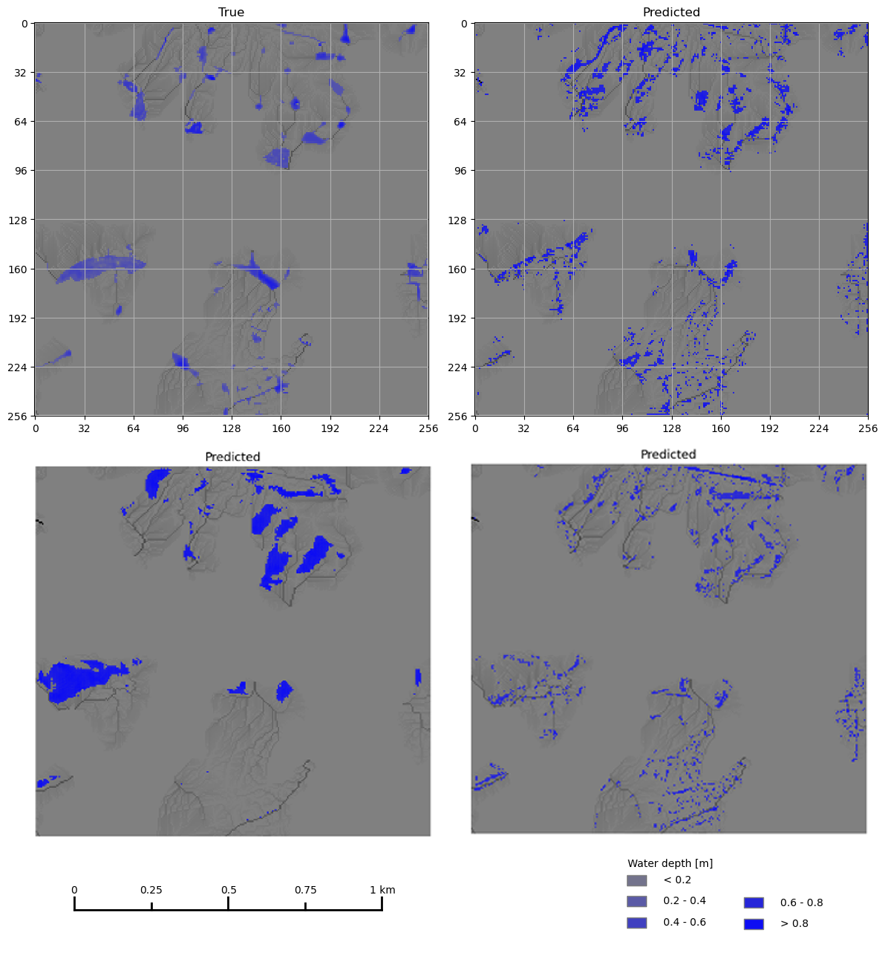
\includegraphics[width=1.0\columnwidth]{assets/res_fig.png}
    \caption{中等或强降雨时正常水深与预测水深}
    \label{res_1}
\end{figure}

\begin{figure}
    \centering
    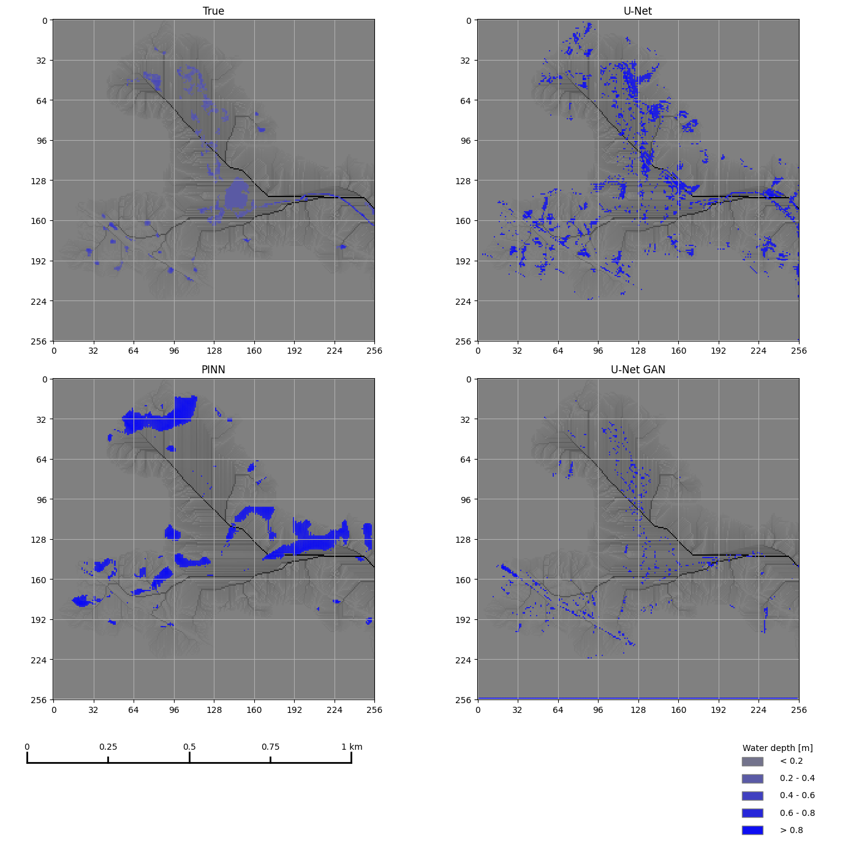
\includegraphics[width=1.0\columnwidth]{assets/res_fig2_2.png}
    \caption{弱降雨时正常水深与预测水深}
    \label{res_2}
\end{figure}

\section{结果分析}

\subsection{模型架构改进对预测效果的影响}

分析FINN的推理结果，我们发现UNet在中强降雨条件下能较好把握内涝的空间分布，但对水深的预测存在较大偏差；PI-UNet显著优化了水深的连续性，但牺牲了生成准确性和可解释性；UNet-GAN则在降雨-径流关系上更为灵敏，能够精准捕捉内涝的分布和水深，在多尺度涝区的预测中表现出了明显的优势。

从图\ref{res_1}的中等或强降雨的案例中可以直观地对比得到，在中等或者强降雨条件下，当真实内涝较为显著时，三种模型架构对于内涝的基本空间分布均有一定的把控，可以大述判断出内涝的发生地点和潜在水深，精度约在125米左右。但是对于125米以内的内涝分布和水深预测的精度有较大差异：UNet对分布有更加激进的预测，其对应位置的水深也有较明显点高估；PI-UNet虽然融合了物理机制，在水深的连续性上有所优化，但是也带来了相当程度的预测错误；UNet-GAN虽然生成结果仍然较为离散，但其分布与真值基本一致，具有把握到10米级的洪涝情况的潜力。

对于弱降雨时模型的预测有更严峻的考验，如何灵敏地把握降雨特征并在原始坑洼上生成小尺度涝区，是衡量模型在洪涝预测中的表现的关键。图\ref{res_2}的结果表明，UNet和PI-UNet无法准确降低洪涝水量。另外，PI-UNet保持了生成的连续性，但其内涝积水的生成结果出现了明显失真的情况，并不符合真实的洪涝情景。而相对应地，UNet-GAN对降雨-径流关系更加灵敏，在生成时综合了水量和空间上的坑洼关系，在水深和分布的预测上都表现出了稳定的优越性。

\subsection{通道权重分析}

在模型训练完成后，我们可以进一步分析模型各通道在进行预测时的权重。

不妨假设FINN是一个正则性质良好的算符，是非病态的，具备较好的连续性，且满足较好的Lipschitz条件。基于这一假设，我们尝试计算FINN各通道的第一特征值。
\begin{equation}
    [FINN]_i X_i = \lambda_i X_i \quad i = 1, 2, 3, 4, 5, 6
\end{equation}

上式中，i指标代表通道，表示输入地形数据的6个特征。我们认为$\vert \lambda_i \vert$，即算符在该通道上的第一特征值的模长，能够代表各地形特征（各通道）在进行预测时的权重。

由于对整个FINN进行特征值计算复杂度较高，我们截取了模型的第一个卷积层作为代理。结果如图\ref{weights}所示。

\begin{figure}[htbp]
\centering
\subfigure[UNet]{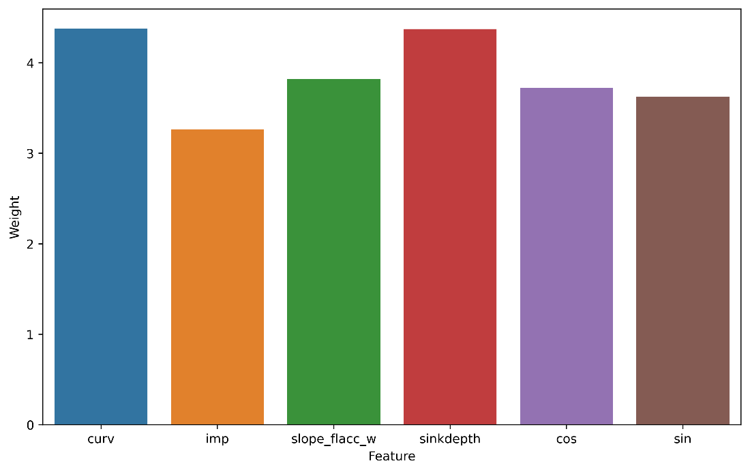
\includegraphics[width=0.40\columnwidth]{./assets/weights_UNet.png}}
\subfigure[PI-UNet]{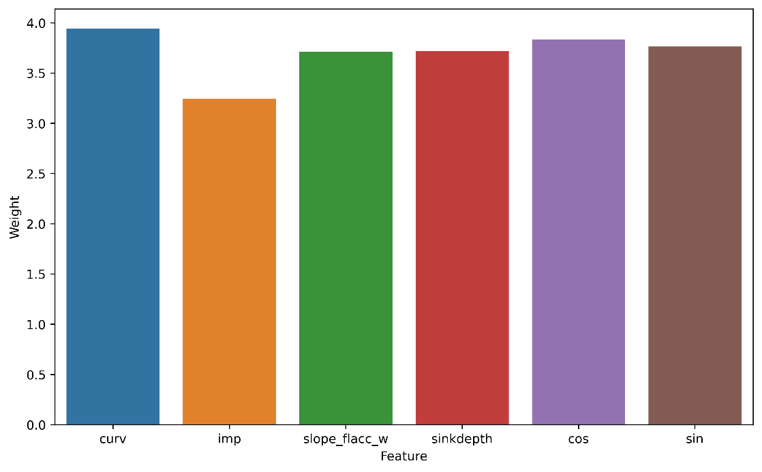
\includegraphics[width=0.40\columnwidth]{./assets/weights_PINN.png}}
\caption{FINN的通道权重分布}
\label{weights}
\end{figure}

可以看出，PI-UNet的通道权重分布相对更为均匀，这是因为我们添加的物理约束强迫FINN在进行预测时必须更加综合地考虑多种特征，而不是更加关注较为显著的特征。而在各个特征中，地表曲率（curv）是最为重要的，而地表透水性是相对不重要的（imp），这与我们在水力学中的传统理论相符合。

通过通道权重分析，我们进一步证明了FINN进行预测的合理性，同时也较为直观地展示了物理约束在模型架构中起到的重要作用。

\section{总结}

本研究提出了一种基于物理信息神经网络的城市内涝水深建模方法。我们结合了深度学习与传统水力学理论，创新性地引入了U-Net架构，GAN等，提出了具备优异预测精度和可靠性的FINN模型，有望克服复杂城市地形下的洪水内涝水深预测问题中的诸多挑战。

实验结果表明，UNet架构在中强降雨条件下能够较好地把握内涝的空间分布，但存在水深预测偏差的问题。PI-UNet通过引入物理约束，显著优化了水深的连续性，但生成的准确性有所牺牲。相比之下，UNet-GAN在多尺度涝区的预测中表现出明显的优势，能够更灵敏地捕捉降雨-径流关系，提供更为准确的水深和分布预测。

我们相信，FINN模型将为城市的防洪规划提供坚实的数据支持，为城市内涝预测问题提供一条创新且高效的解决途径，同时也可以作为水力学和深度学习交叉研究的参考。未来，我们将着眼于模型结构的进一步优化和更多物理信息与数据的嵌合两方面继续研究，以提升FINN在复杂环境中的预测精度、适应性和泛化能力。

\bibliographystyle{apalike}
\bibliography{bibliography}

\end{document}
